
%(BEGIN_QUESTION)
% Copyright 2011, Tony R. Kuphaldt, released under the Creative Commons Attribution License (v 1.0)
% This means you may do almost anything with this work of mine, so long as you give me proper credit

A pneumatic DP transmitter measures the flow of gasoline through a an orifice plate, using a separate square root extractor relay to characterize the signal so that it may be displayed linearly on the receiver gauge (FI-20):

$$\includegraphics[width=15.5cm]{i03441x01.eps}$$

Based on other flow-measuring devices in this process, operations personnel have determined the actual flow rate through this pipe is 171 gallons per minute.  FI-20, however, registers a flow of 184 gallons per minute.  Based on the data you see in this illustration, determine the location of the calibration error.

\underbar{file i03441}
%(END_QUESTION)





%(BEGIN_ANSWER)

The error lies with the indicator (FI-20).

%(END_ANSWER)





%(BEGIN_NOTES)


%INDEX% Calibration errors, identifying
%INDEX% Measurement, flow: square root characterized pressure transmitter

%(END_NOTES)

